\chapter{はじめに}

\section{TuneEditor 4.xとは?}

 TuneEditorとは、英語の文字表現や発音記号(音声記号)だけでは表しきれないプロソディー(音の強弱や高低、長短)を視覚情報として表記するためのアプリケーションであり、イギリスの音声学研究におけるロンドン学派の表記法を簡単に入力できるようにすることを第1の目的にしています。

サポートしている表記法は、英語の文章中に付加記号(Tone Stress Mark:TSM)を記述する方式(以下、\textsf{TSM表記}と略)と、音の高低を表す上下線の間に黒いドット(音の高低を高さで、音の強弱を大きさで表し、音の長短/リズムを(ざっくりと)その間隔で表現する)を記述して表現する方式(以下、\textsf{行間表記}と略)です。

なお入力後のイメージはjpeg形式の画像ファイルとして、また作業中の内容をプロジェクトファイル(拡張子は「.ti4」)として保存できます。
\smallskip

\begin{figure}[htbp]
\begin{center}
	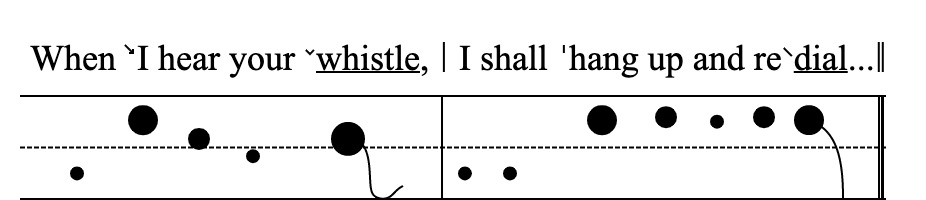
\includegraphics[width=12cm]{TuneEditorSample.jpeg}
 \end{center}
 \caption{TuneEditorの出力サンプル}
 \label{sampleImage}
\end{figure}

\section{動作環境}

 このアプリケーションはブラウザーアプリです。
動作確認はmacOS上のGoogle Chromeで行っていますが、基本的にはモダンなブラウザーであれば動作する\textsf{はず}です。

\textbf{追記:}FireFoxではabout:configの画面で

\begin{quote}
\begin{verbatim}
dom.textMetrics.fontBoundingBox.enabled=true
\end{verbatim}
\end{quote}

と設定しておく必要があります。

また、ディスプレイ画面は横幅900ピクセル以上がおすすめですが、ブラウザーの縮小表示機能を使えばもう少し小さいウィンドウ領域でも使用できるはずです。


\section{ライセンス}

 本アプリケーションはMIT Licenseを採用したフリーソフトウェアであり、無償で利用することができます(利用の結果で発生する問題等については無保証ですが、希望を述べてもらうと対応するかもしれません \verb+^^;+)。
